%%%%%%%%%%%%%%%%%%%%%%%%%%%%%%%%%%%%%%%%%%%%%%%%%%%%%
      %%%%%%%%%%%%% Phases of Matter %%%%%%%%%%%%
%%%%%%%%%%%%%%%%%%%%%%%%%%%%%%%%%%%%%%%%%%%%%%%%%%%%%
\section{Phases of Matter}

\begin{frame}
    \frametitle{Phases os matter}
    In the very heart of the classification of these phase lies
    the concept of symmetry. Therefore, the phase transitions
    are related to symmetry-breaking processes.

    \begin{columns}

    \column{0.3\textwidth}
    On a daily basis:
    \begin{itemize}
        \item Plasma
        \item Gases
        \item Liquids
        \item Solids
    \end{itemize}

    \column{0.70\textwidth}
    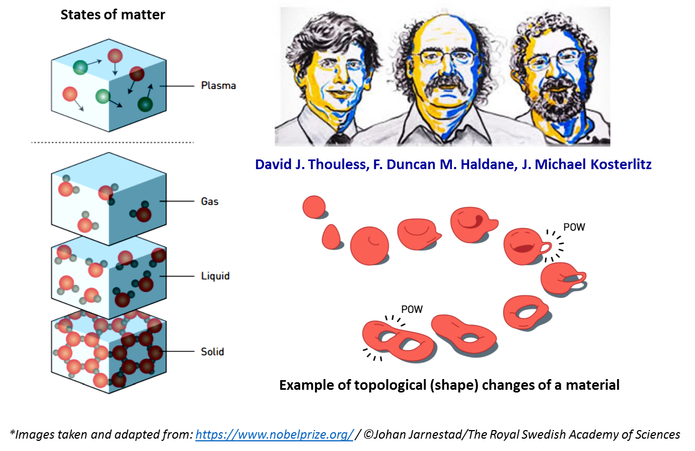
\includegraphics[width=1\textwidth]{/home/marcos/topological_insulator_presentation/Topological-insulator-presentation/phases_of_matter/nobel_with_mug_doughnut.png}

    \end{columns}

\end{frame}

\begin{frame}

    \frametitle{Symmetry and order}

    \begin{columns}

    \column{0.5\textwidth}


    \column{0.5\textwidth}

    \end{columns}

\end{frame}


%%%%%%%%%%%%%%%%%%%%%%%%%%%%%%%%%%%%%%%%%%%%%%%%%%%%%
      %%%%%%%  Quantum Phases of Matter %%%%%%%
%%%%%%%%%%%%%%%%%%%%%%%%%%%%%%%%%%%%%%%%%%%%%%%%%%%%%
\section{Quantum phases of Matter}

\begin{frame}
\frametitle{Diferenças Finitas (1D)}


    \begin{empheq}[box={\mymath}]{equation*}
    i\hbar \frac{\partial\psi(x,t)}{\partial t} = \left[ -\frac{\hbar^2}{2m_e} \frac{\partial^2}{\partial x^2} + V(x)\right]\psi(x,t)
    \end{empheq}


    %\pause

    \begin{columns}

    \column{0.4\textwidth}
    \begin{empheq}[box=\tcbhighmath]{align*}
    x \rightarrow x_m &\equiv m \Delta x\\
    t \rightarrow t_n &\equiv n \Delta t \\
    \\
    \psi(x_m,t_n) &\equiv \psi_{m,n}
    \end{empheq}

    \column{0.6\textwidth}

    %\onslide<3->{
    \begin{empheq}[box={\mymath}]{align*}
    \left.\frac{\partial^2 \psi}{\partial x^2}\right|_{x_m,t_n} &\approx \frac{\psi_{m+1,n}+\psi_{m-1,n}-2\psi_{m,n}}{\Delta x^2}\\
    \\
    \left.\frac{\partial \psi}{\partial t}\right|_{x_m,t_n} &\approx \frac{\psi_{m,n+1} - \psi_{m,n}}{\Delta t}
    \end{empheq}
    %}

    \end{columns}

\end{frame}


%%%%%%%%%%%%%%%%%%%%%%%%%%%%%%%%%%%%%%%%%%%%%%%%%%%%%
      %%%%% Topological  Phases of Matter %%%%
%%%%%%%%%%%%%%%%%%%%%%%%%%%%%%%%%%%%%%%%%%%%%%%%%%%%%
\section{Topological phases of Matter}




\begin{frame}
    \frametitle{Topological phases of matter}

    Topology $=$ (\textgreek{t'opos}) $+$ (\textgreek{l'ogos})
    $=$ place $+$ study
    

    % \begin{columns}
    %
    % \column{0.5\textwidth}


    % \column{0.5\textwidth}
    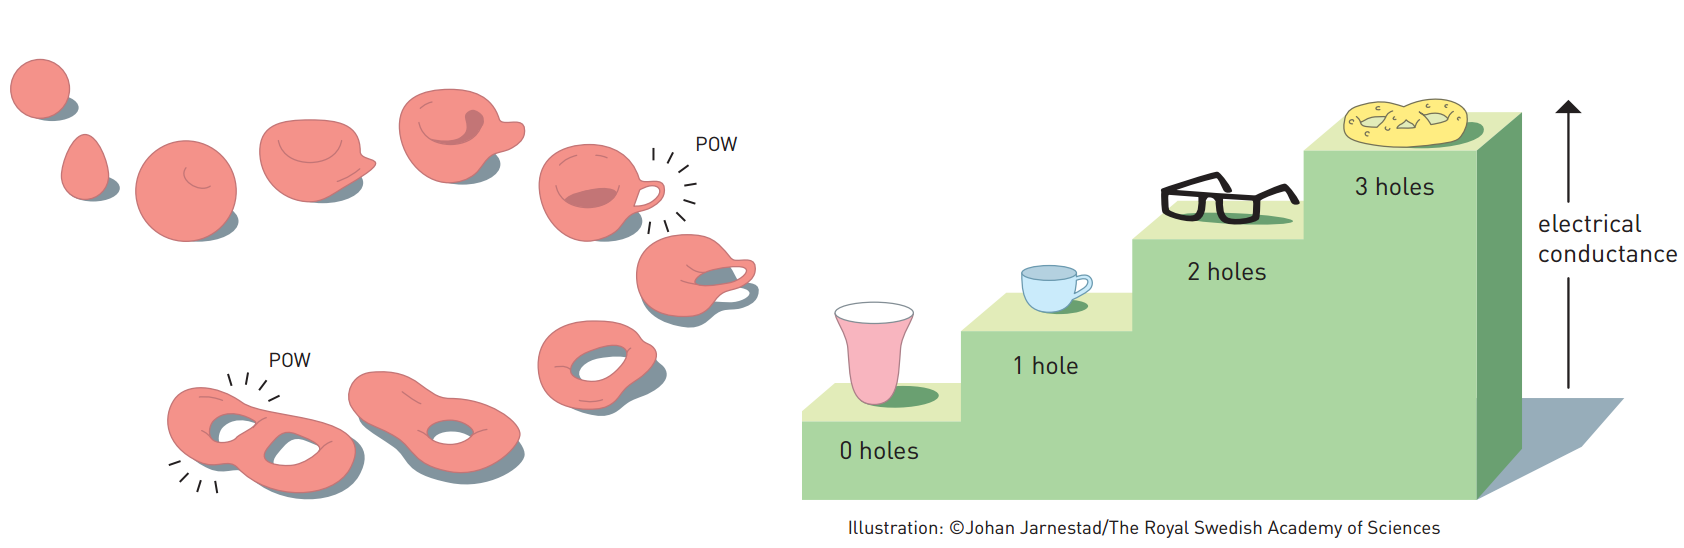
\includegraphics[width=1\textwidth]{/home/marcos/topological_insulator_presentation/Topological-insulator-presentation/phases_of_matter/scale_of_genus_number.png}

    % \end{columns}

\end{frame}



%%%%%%%%%%%%%%%%%%%%%%%%%%%%%%%%%%%%%%%%%%%%%%%%%%%%%
      %%%%%%%%%%  Why does it matters %%%%%%%%
%%%%%%%%%%%%%%%%%%%%%%%%%%%%%%%%%%%%%%%%%%%%%%%%%%%%%
\section{Why does it matters?}

\begin{frame}
    \frametitle{Phases os matter}
%O estudo das chamadas fases topógicas da matéria possuem
%motivações que vão desde a pesquisa básica até a aplicação
%na engenharia de dispositivos:

    \begin{columns}

    \column{0.45\textwidth}
    On a daily basis:
    \begin{itemize}
        \item Gases;
        \item Liquids;
        \item Solids;
        \item Plasma.
    \end{itemize}

    \column{0.7\textwidth}
    % \includegraphics[width=1\textwidth]{/home/marcos/Dropbox/images_presentations/spin_orbitronics.png}
    %
    % {\tiny
    % Manchon, Aurelien, et al. "New perspectives for Rashba spin-orbit coupling." arXiv preprint arXiv:1507.02408 (2015)


    \end{columns}

\end{frame}
